\documentclass{article}

%table customization, stack overflow 
\usepackage{array}
\newcolumntype{L}[1]{>{\raggedright\let\newline\\\arraybackslash\hspace{0pt}}m{#1}}

\usepackage{enumitem}
\usepackage{graphicx}
\usepackage{booktabs}
\usepackage{url}
\usepackage{hyperref}
\usepackage{fancyhdr}
\pagestyle{fancy}
\begin{document}
\pagenumbering{gobble}
\lhead{Team 6\\ JSTanks\\}
\newpage
\title{JSTanks - Test Report}
\date{October 31, 2016}
\author{Jiahao Li\\LI577\\Student \# \and Pavithran Pathmarajah\\PATHMAP\\001410729 \and Viren Patel\\PATELVH3\\Student \#}

\maketitle

\newpage
\pagenumbering{arabic}
\tableofcontents
\newpage
\section{Revision History}
\subsection{Revision 0}
\begin{table}[h]
\caption{Revision History}
	\begin{tabular}{clc}
		\toprule
		Date & Developer & Change\\
		\midrule
		October 31&Jiahao Li &Initial Draft \\
		October 31&Pavithran Pathmarajah &Initial Draft\\
		October 31&Viren Patel  &Initial Draft\\
	\end{tabular}
\end{table}


\section{General Information}
\subsection{Purpose}
\subsection{Scope}
\subsection{Acronyms, Abbreviations, and Symbols}
\begin{figure}[h]
	\centering
	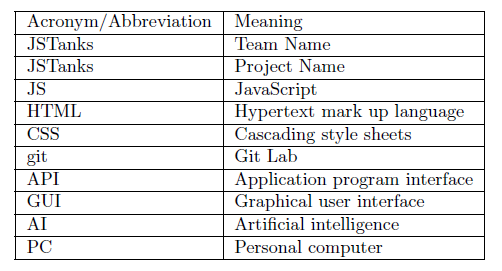
\includegraphics[width=\textwidth]{fig1.png}
	\caption{Acronyms}
\end{figure}

\subsection{Overview of Document}

\section{Plan}
\subsection{Software Description}
JSTanks is a game which allows users enjoy it on a website without downloading it. This game let the user control a tank to fire and move on the map in order to protect its home base and itself from the damage of other tanks'.
\subsection{Test Team}
The test team will consist of Jiahao Li, Pavithran Pathmarajah, Viren Patel and some random players as testers. Jiahao Li, Pavithran Pathmarajah, Viren Patel will split the entire testing which cover all different types of tests. The random player will test the performance of the game and give feedbacks to the development team.
\subsection{Automated Testing Approach}
\subsection{Testing Tools}
\subsection{Testing Schedule}

\section{System Test Description}
\subsection{Tests for Functional Requirements}
\subsubsection{HTML file test}
Name:  Creating new browser by html file \newline
Description: Test if the executable HTML file creates a new browser window. \newline
Type: Unit test (dynamic, manual, black box) \newline
Initial State:  A html file in the operating system \newline
Input: Click the html file \newline
Output: A new browser \newline
Pass: A new browser pops up. \newline

\subsubsection{Standby state test}
Name:  Standby state\newline
Description: Test if the game has a standby state in which it waits for user input. \newline
Type: Unit test (static, automated, black box) \newline
Initial State: A new browser \newline
Input: -- \newline
Output: The standby state of the game \newline
Pass:The new browser with the game menu in it. \newline

\subsubsection{Menu test}
Name:  Menu representation\newline
Description: est if the menu with four sections which are game, pause/continue, level and introduction shows up in the standby state. \newline
Type: Unit test (dynamic, manual, black box) \newline
Initial State: A new browser \newline
Input: -- \newline
Output: The standby state of the game\newline
Pass: The menu with four sections is represented in the standby state. \newline

\subsubsection{The game section of the menu test}
Name: Menu of game section\newline
Description: Test if the sub menu of game section which has choices of starting a new game and quit shows up when the game section is clicked. \newline
Type: Unit test (dynamic, manual, black box) \newline
Initial State: Menu in the standby state \newline
Input: Click the game section of the menu \newline
Output: The sub menu \newline
Pass:The sub menu with choice of starting a new game and quit. \newline

\subsubsection{The pause section of the menu test}
Name: Menu of pause and continue\newline
Description: Test if the sub menu of pause/continue section which has choices of pause and continue shows up when the pause/continue section is clicked. \newline
Type: Unit test (dynamic, manual, black box) \newline
Initial State:  Menu in the standby state \newline
Input: Click the pause/continue section of the menu \newline
Output: The sub menu  \newline
Pass: The sub menu with choice of pause and continue. \newline

\subsubsection{The level section of the menu test}
Name:  Menu of level\newline
Description: Test if the sub menu of level section which has choices of level 1, level 2, and level 3 shows up when the level section is clicked. \newline
Type: Unit test (dynamic, manual, black box) \newline
Initial State: Menu in the standby state \newline
Input: Clickthe level section of the menu\newline
Output: The sub menu\newline
Pass: The sub menu with choice of level1, level 2 and level 3. \newline

\subsubsection{Game start test}
Name:  Start the game\newline
Description: Test if the game shall be reset and start when [starting a new game] is clicked. \newline
Type: Unit test (dynamic, manual, black box) \newline
Initial State:  The sub menu of the game section \newline
Input: Click the choice of starting a new game \newline
Output: The standby state of the game\newline
Pass: The standby state of the game with all objects on their initial position on the map. \newline

\subsubsection{Game quit test}
Name:  Quit the game\newline
Description: Test if the game comes to the end state that the GUI turns into black with only the menu on it when the choice of quit is clicked. \newline
Type: Unit test (dynamic, manual, black box) \newline
Initial State:  The running state of the game \newline
Input: Click the choice of quit\newline
Output: the end state of the game  \newline
Pass: The game comes to the end state that the GUI turns into black with only the menu on it. \newline

\subsubsection{Game pause test}
Name:  Pause the game\newline
Description: Test if the game comes to the pause state when the choice of pause is clicked. \newline
Type: Unit test (dynamic, manual, black box) \newline
Initial State: The running state of the game \newline
Input: Click the choice of pause \newline
Output: The pause state of the game\newline
Pass: The game comes to the pause state that all stuff in the game freeze and stay in the temporal positions. \newline

\subsubsection{Game continue test 0}
Name:  Continue the game\newline
Description: Test if the game comes back to the running state from the pause state when the choice of continue is clicked in the pause state. \newline
Type: Unit test (dynamic, manual, black box) \newline
Initial State: The pause state of the game\newline
Input: Click the choice of continue \newline
Output: The running state of the game\newline
Pass: All stuff frozen in the pause state are activated and back into the routine. \newline

\subsubsection{Game continue test 1}
Name:  Continue the game in the running state\newline
Description: Test if there is any effect on the game when the choice of continue is clicked in the running state. \newline
Type: Unit test (dynamic, manual, black box) \newline
Initial State: The running state of the game \newline
Input: Click the choice of continue \newline
Output: The running state of the game \newline
Pass: No effect on the running state. \newline

\subsubsection{AI test}
Name:  The routine of AI e\newline
Description: Test if the AI controls tanks to move and fire randomly. \newline
Type: Unit test (dynamic, automated, white box) \newline
Initial State: The running state of the game \newline
Input: -- \newline
Output: The routine of tanks controlled by the AI \newline
Pass: The tanks controlled by the AI move and fire randomly. \newline

\subsubsection{Level test}
Name:  Levels of the game\newline
Description: Test if the moving speed of tanks controlled by the AI change when level 1, level 2 or level 3 is clicked. \newline
Type: Unit test (dynamic, automated, black box) \newline
Initial State:  The running state of the game \newline
Input: Click the choice of different level\newline
Output: The different speed of movements of tanks controlled by the AI \newline
Pass: The higher the level is, the higher the speed of movements of tanks controlled by the AI is. \newline

\subsubsection{Default level test}
Name:  The default level of the game\newline
Description: Test if the level 1 is chosen as the default speed of tanks controlled by the AI when the game starts. \newline
Type: Unit test (static, automated, white box) \newline
Initial State:  Thethe standby state of the game \newline
Input: Click the choice of starting a new game\newline
Output: The game starts with tanks controlled by the AI moving in the lowest speed\newline
Pass: The game starts with tanks controlled by the AI moving in the lowest speed. \newline

\subsubsection{Information test}
Name:  The information of the game\newline
Description: Test if The window with the information of the game in it pops up when the section of introduction is clicked. \newline
Type: Unit test (dynamic, manual, black box) \newline
Initial State:  The menu with four sections \newline
Input: Click the choice of different level\newline
Output: The window with information in it \newline
Pass:  The window with information in it pops up. \newline

\subsubsection{Movement test}
Name:  The movement of the tank controlled by the user\newline
Description: Test if the tank controlled by the user moves left, right, up or down when the left, right, up or down key on the keyboard is pressed. \newline
Type: Unit test (dynamic, manual, black box) \newline
Initial State:  The running state of the game \newline
Input: Press the left, right, up or down key on the keyboard\newline
Output: The movement of the tank controlled by the user \newline
Pass: The tank moves to the correct direction one step according to the key pressed by the user every time. \newline

\subsubsection{Continuous movement test}
Name:  The continuous movement of the tank controlled by the user\newline
Description: Test if the tank controlled by the user keeps moving in the direction of left, right, up or down when the left, right, up or down key on the keyboard is held. \newline
Type: Unit test (dynamic, manual, black box) \newline
Initial State:  The running state of the game \newline
Input: Hold the left, right, up or down key on the keyboard\newline
Output: The continuous movement of the tank controlled by the user\newline
Pass:  The tank keeps moving in the correct direction according to the key held by the user until the user release the key. \newline

\subsubsection{Bullet launch test}
Name:  Launch the bullet\newline
Description: Test if the tank controlled by the user launches a bullet when the user press the space on the keyboard. \newline
Type: Unit test (dynamic, manual, black box) \newline
Initial State: The running state of the game \newline
Input: Press the space on the keyboard\newline
Output: The tank controlled by the user launches a bullet in the direction it faces to \newline
Pass: The tank controlled by the user launches a bullet in the direction it faces to. \newline

\subsubsection{Bullet movement test}
Name:  The movement the bullet\newline
Description: Test if the bullet keep moving in the same direction after being launched. \newline
Type: Unit test (dynamic, automated, black box) \newline
Initial State:  The bullet is launched \newline
Input: --\newline
Output: The bullet keep moving in the same direction which it launched to\newline
Pass:  The bullet keep moving in the same direction which it launched to. \newline

\subsubsection{Bullet disappearance test}
Name:  The bullet disappearance \newline
Description: Test if the bullet disappears when it hits the tank, wall, steel, home base or the boundary of the map. \newline
Type: Unit test (dynamic, automated, black box) \newline
Initial State:  the bullet hits a wall. a steel, the home base of the boundary of the map\newline
Input: --\newline
Output: The bullet disappear\newline
Pass: The bullet disappears when it hits the tank, wall, steel, home base or the boundary of the map. \newline

\subsubsection{Wall hit test}
Name:  The wall hit by the bullet\newline
Description: Test if the wall disappears when it is hit by the bullet. \newline
Type: Unit test (dynamic, automated, black box) \newline
Initial State:  The wall is hit by the bullet \newline
Input: --\newline
Output: The wall disappears \newline
Pass:  The wall disappears immediately when it is hit by the bullet. \newline

\subsubsection{Steel hit test 0}
Name:  The steel hit by the bullet twice\newline
Description: Test if the steel stays the same when it is hit by the bullet twice. \newline
Type: Unit test (dynamic, automated, black box) \newline
Initial State:  The steel is hit by the bullet \newline
Input: --\newline
Output: The steel stays the same \newline
Pass:  The steel stays the same when it is hit by the bullet twice. \newline

\subsubsection{Steel hit test 1}
Name:  the steel hit by the bullet at the third time\newline
Description: Test if the wall disappears when it is hit by the bullet at the third time. \newline
Type: Unit test (dynamic, automated, black box) \newline
Initial State:  The steel is hit by the bullet \newline
Input: --\newline
Output: The steel disappears \newline
Pass:   The steel disappears when it is hit by the bullet at the third time. \newline


\subsubsection{Enemy tanks hit test}
Name:  The tank controlled by the AI hit by the bullet\newline
Description: Test if the tank controlled by the AI disappears when it is hit by the bullet. \newline
Type: Unit test (dynamic, automated, black box) \newline
Initial State:  The tank controlled by the AI is hit by the bullet \newline
Input: --\newline
Output: The tank controlled by the AI disappears \newline
Pass: The tank controlled by the AI disappears when it is hit by the bullet. \newline


\subsubsection{Home base hit test 0}
Name:  The home base hit by the bullet for first four times\newline
Description: Test if the home base stays the same when it is hit by the bullet for first four times. \newline
Type: Unit test (dynamic, automated, black box) \newline
Initial State:  The home base is hit by the bullet \newline
Input: --\newline
Output: The home base stays the same \newline
Pass:  The home base stays the same when it is hit by the bullet for first four times. \newline


\subsubsection{Home base hit test 1}
Name: The home base hit by the bullet at the fifth time\newline
Description: Test if the home base disappears when it is hit by the bullet  at the fifth time. \newline
Type: Unit test (dynamic, automated, black box) \newline
Initial State:  The home base is hit by the bullet \newline
Input: --\newline
Output: The home base disappears\newline
Pass: The home base disappears when it is hit by the bullet  at the fifth time. \newline

\subsubsection{User tank hit test 0}
Name: The tank controlled by the user hit by the bullet for first four times\newline
Description: Test if the tank controlled by the user stays the same when it is hit by the bullet for first four times,. \newline
Type: Unit test (dynamic, automated, black box) \newline
Initial State:  The tank controlled by the user is hit by the bullet \newline
Input: --\newline
Output: The tank controlled by the user stays the same \newline
Pass: The tank controlled by the user stays the same when it is hit by the bullet for first four times. \newline

\subsubsection{User tank hit test 1}
Name:  The tank controlled by the user hit by the bullet at the fifth time\newline
Description: Test if the tank controlled by the user disappears when it is hit by the bullet at the fifth time. \newline
Type: Unit test (dynamic, automated, black box) \newline
Initial State:  The tank controlled by the user is hit by the bullet \newline
Input: --\newline
Output: The tank controlled by the user disappears \newline
Pass: The tank controlled by the user disappears when it is hit by the bullet at the fifth time. \newline

\subsubsection{Game over test 0}
Name:  the tank is destroyed\newline
Description: Test if the game comes to the end state when the tank controlled by the user disappears. \newline
Type: Unit test (dynamic, automated, black box) \newline
Initial State:  The tank controlled by the user disappears\newline
Input: --\newline
Output: The end state of the game \newline
Pass:  The game comes to the end state that the GUI turns into black with only the menu on it. \newline

\subsubsection{Game over test 1}
Name:  The home base is destroyed\newline
Description: Test if the game comes to the end state when the home base disappears. \newline
Type: Unit test (dynamic, automated, black box) \newline
Initial State:  The home base disappears \newline
Input: --\newline
Output: The end state of the game \newline
Pass:  The game comes to the end state that the GUI turns into black with only the menu on it. \newline





\subsection{Tests for Nonfunctional Requirements}
\subsubsection{Area of Testing1}
\subsubsection{Area of Testing2}




\section{Tests for Proof of Concept}
The proof of concept forJSTanks was to demonstrate a block moving across the screen in up, down, left, and right directions according to the user input from the keyboard. In addition, boundaries had to be set so that the block does not go off-screen. JSTanks was successfully able to present this during the proof of concept demonstration. The testing measures included functional dynamic testing as follows:
\subsection{Display}
Name: Display block\newline
Description: Test if the block is successfully displayed on the web screen once the corresponding html file is launched.\newline
Type: Unit Test (dynamic, manual, black box)\newline
Initial State: Empty white screen\newline
Input: Not Applicable\newline
Output: A block\newline
Pass: A block is displayed on the screen
\subsection{Movement}
Name: Block movement\newline
Description: Test if the block’s position is updated after the user input.\newline
Type: Unit Test (dynamic, manual, black box)\newline
Initial State: block displayed on screen\newline
Input: Up, down, left, or right key on the keyboard\newline
Output: The block moves accordingly\newline
Pass: The tank’s position is updated by the specified value in the correct direction.
\subsection{Boundaries}
Name: Screen Boundary\newline
Description: Test if the block stays in bounds of the screen.\newline
Type: Unit Test (dynamic, manual, black box)\newline
Initial State: block displayed on screen\newline
Input: Any one of up, down, left or right key on the keyboard until the block is at the edge of the screen in the according side.\newline
Output: The block stays on the screen near the corresponding edge and does not go off-screen.\newline
Pass: The block stays within the screen even though the input tries to force it off-screen.




\section{Comparison to Existing Implementation}
The open source game software we are working on is simply a Java application in its existent form. We are uploading the same game on a web browser which requires a different programming language altogether. As a result, we have not been able to use any existing code and have had to program the game completely from scratch. We have also not looked into the Java code to learn its implementation style or use any ideas for specific functions. Therefore, any similarities between our code and the existing code are coincidental. \\ \\
The major difference between the two implementations is that we have HTML, and CSS files in addition to the JavaScript source code which are required for any kind of web development. The existing code works with multiple classes representing different aspects of the game which can be seen in our code as well. However, it has more classes, three of them which are main method classes which can be explained by the programming language used. Our implementation has no main method or class, but instead the HTML file is used as the main class which drives the whole game. Another important difference is the style of programming; the existing implementation has made use of threads which we have not as we are still learning to work with JavaScript. The use of object oriented programming is evident in both implementations. For example, objects for tanks, bots, and barriers are included in both. 





\section{Unit Testing Plan}
\subsection{Unit testing for internal functions}
\subsubsection{Wall type test}
Name:  Ask for the type of the wall\newline
Description: Test if the program return the type of the wall when you ask for it. \newline
Type: Unit test (dynamic, automated, white box) \newline
Initial State:  The object of wall is created \newline
Input: wall.type()\newline
Output: BARRIER  \newline
Pass:   The program return the type BARRIER when we call the wall.type() function. \newline

\subsubsection{Steel type test}
Name:  Ask for the type of the steel\newline
Description: Test if the program return the type of the steel when you ask for it. \newline
Type: Unit test (dynamic, automated, white box) \newline
Initial State:  The object of steel is created \newline
Input: steel.type()\newline
Output: BARRIER\newline
Pass:  The program return the type BARRIER when we call the wall.type() function. \newline

\subsubsection{Home base type test}
Name:  Ask for the type of the home base\newline
Description: Test if the program return the type of the hoem base when you ask for it. \newline
Type: Unit test (dynamic, automated, white box) \newline
Initial State:  The object of home base is created \newline
Input: homebase.type()\newline
Output: BARRIER\newline
Pass:  The program return the type BARRIER when we call the wall.type() function. \newline

\subsubsection{Wall draw test}
Name:  Draw the wall on the game board\newline
Description: Test if the image of the wall shows up on the position we set on the game board in the right size when we call this function. \newline
Type: Unit test (dynamic, automated, white box) \newline
Initial State:  The game board with no image on the position (startX,startY) \newline
Input: wall.draw(canvas,startX,startY,tileSize,t)\newline
Output: The image of the wall shows up on the position (startX,startY) of the game board\newline
Pass:  The image of the wall shows up on the position (startX,startY) of the game board in the tileSize. \newline

\subsubsection{Steel draw test}
Name:  Draw the steel on the game board\newline
Description: Test if the image of the steel shows up on the position we set on the game board in the right size when we call this function. \newline
Type: Unit test (dynamic, automated, white box) \newline
Initial State:  The game board with no image on the position (startX,startY) \newline
Input: steel.draw(canvas,startX,startY,tileSize,t)\newline
Output: The image of the steel shows up on the position (startX,startY) of the game board\newline
Pass:  The image of the steel shows up on the position (startX,startY) of the game board in the tileSize. \newline

\subsubsection{Home base draw test}
Name:  Draw the home base on the game board\newline
Description: Test if the image of the home base shows up on the position we set on the game board in the right size when we call this function. \newline
Type: Unit test (dynamic, automated, white box) \newline
Initial State:  The game board with no image on the position (startX,startY) \newline
Input: homebase.draw(canvas,startX,startY,tileSize,t)\newline
Output: The image of the home base shows up on the position (startX,startY) of the game board\newline
Pass:  The image of the home base shows up on the position (startX,startY) of the game board in the tileSize. \newline

\subsubsection{Wall hit test}
Name:  Hit the wall\newline
Description: Test if the program decreases the points of strength of the wall after the wall is hit. \newline
Type: Unit test (dynamic, automated, white box) \newline
Initial State:  The remaining points of strength of the wall\newline
Input: wall.hit()\newline
Output: --\newline
Pass:  One point of strength of the wall is decreased after the wall is hit. \newline

\subsubsection{Steel hit test}
Name:  Hit the steel\newline
Description: Test if the program decreases the points of strength of the steel after the steel is hit. \newline
Type: Unit test (dynamic, automated, white box) \newline
Initial State:  The remaining points of strength of the steel\newline
Input: steel.hit()\newline
Output: --\newline
Pass:  One point of strength of the wall is decreased after the steel is hit. \newline

\subsubsection{Home base hit test}
Name:  Hit the home base\newline
Description: Test if the program decreases the points of strength of the home base after the home base is hit. \newline
Type: Unit test (dynamic, automated, white box) \newline
Initial State:  The remaining points of strength of the home base\newline
Input: homebase.hit()\newline
Output: --\newline
Pass:  One point of strength of the wall is decreased after the home base is hit. \newline

\subsubsection{Wall health get test}
Name:  Get health of the wall\newline
Description: Test if the program return the remaining points of strength of the wall after calling this function. \newline
Type: Unit test (dynamic, automated, white box) \newline
Initial State:  the object of wall\newline
Input: wall.getHealth()\newline
Output: The remaining points of strength of the wall\newline
Pass:  Return the remaining points of strength of the wall after calling this function. \newline

\subsubsection{Steel health get test}
Name:  Get health of the steel\newline
Description: Test if the program return the remaining points of strength of the steel after calling this function. \newline
Type: Unit test (dynamic, automated, white box) \newline
Initial State:  the object of steel\newline
Input: steel.getHealth()\newline
Output: The remaining points of strength of the steel\newline
Pass:  Return the remaining points of strength of the steel after calling this function. \newline

\subsubsection{Home base health get test}
Name:  Get health of the home base\newline
Description: Test if the program return the remaining points of strength of the home base after calling this function. \newline
Type: Unit test (dynamic, automated, white box) \newline
Initial State:  the object of home base\newline
Input: homebase.getHealth()\newline
Output: The remaining points of strength of the home base\newline
Pass:  Return the remaining points of strength of the home base after calling this function. \newline

\subsubsection{Wall position get test}
Name:  Get the position of the wall\newline
Description: Test if the program return the remaining points of strength of the wall after calling this function. \newline
Type: Unit test (dynamic, automated, white box) \newline
Initial State:  the object of wall has already be drawn\newline
Input: wall.getPosition()\newline
Output: The position of the wall\newline
Pass:  Return the position (x,y) of the wall after calling this function. \newline

\subsubsection{Steel position get test}
Name:  Get the position of the steel\newline
Description: Test if the program return the remaining points of strength of the steel after calling this function. \newline
Type: Unit test (dynamic, automated, white box) \newline
Initial State:  the object of steel has already be drawn\newline
Input: steel.getPosition()\newline
Output: The position of the steel\newline
Pass:  Return the position (x,y) of the steel after calling this function. \newline

\subsubsection{Home base position get test}
Name:  Get the position of the home base\newline
Description: Test if the program return the remaining points of strength of the home base after calling this function. \newline
Type: Unit test (dynamic, automated, white box) \newline
Initial State:  the object of home base has already be drawn\newline
Input: homebase.getPosition()\newline
Output: The position of the home base\newline
Pass:  Return the position (x,y) of the home base after calling this function. \newline

\subsubsection{Tank Constructor Test}
Name: Tank Constructor Testing\newline
Description: Test if a tank object is created with the specified attributes when the constructor is called.\newline
Type: Unit Test (dynamic, automated, white box)\newline
Initial State: Not Applicable\newline
Input: Tank tankObject = new Tank(<initial values>)\newline
Output: Not Applicable \newline
Pass: The following methods work on the tankObject created here.\newline

\subsubsection{Tank Draw Test}
Name: Tank Graphics Testing\newline
Description: Test if the image of the tank shows up at the position set by the game board when the function is called.\newline
Type: Unit Test (dynamic, automated, white box)\newline
Initial State: The game board with no image on the position (startX, startY)\newline
Input: tankObject.draw(canvs, startX, startY, tileSize)\newline
Output: The image of the tank appears on the position (startX, startY) of the game board.\newline
Pass: The tank is successfully displayed on the correct position on the game board.\newline

\subsubsection{Tank Type Test}
Name: Object Type Testing\newline
Description: Test if the method returns the correct type of object located at the specified location on the game board.\newline
Type: Unit Test (dynamic, automated, white box)\newline
Initial State: A tank object is placed at a certain grid location on the game board.\newline
Input: tankObject.type()\newline
Output: “TANK”\newline
Pass: The program returns “TANK” when tankObject.type() is called.\newline

\subsubsection{Tank Hit Test}
Name: Projectile Impact Testing\newline
Description: Test if the health points of the tank are reduced after the tank has been hit with a projectile.\newline
Type: Unit Test (dynamic, automated, white box)\newline
Initial State: The initial health points of the tank\newline
Input: tankObject.hit()\newline
Output: Not Applicable\newline
Pass: Specified points of the tank’s health are reduced.\newline

\subsubsection{Tank Health Test}
Name: Tank Health Getter Testing\newline
Description: Test if the method returns the correct number of health points for the tank when called upon.\newline
Type: Unit Test (dynamic, automated, white box)\newline
Initial State: A tank object has been created.\newline
Input: tankObject.getHealth()\newline
Output: The number of health points of the tank object.\newline
Pass: The method returns the correct number of health points remaining for the tank object.\newline

\subsubsection{Tank Position Test}
Name: Tank Position Getter Testing\newline
Description: Test if the method returns the current position of the tank object.\newline
Type: Unit Test (dynamic, automated, white box)\newline
Initial State: A tank object has been created and is displayed on the game board.\newline
Input: tankObject.getPosition()\newline
Output: The position of the tank object (x and y co-ordinates)\newline
Pass: The correct position (x and y co-ordinates) of the tank is returned by the method.\newline


\subsection{Unit testing for output files}

\section{Appendix}
\subsection{Symbolic Parameters}
\subsection{Usability Survey Questions}

\newpage
\listoftables
\listoffigures

\end{document}